\documentclass[a4paper,10pt,twocolumn]{article}
\usepackage[utf8]{inputenc}
\usepackage[top=1.8cm,bottom=2.0cm,right=1.35cm,left=1.35cm,columnsep=0.5cm]{geometry}
\usepackage{setspace, url}
\usepackage[natbibapa]{apacite}
\bibliographystyle{apacite}
\usepackage{graphicx}
\usepackage{amsmath}
\usepackage{amsfonts}
\usepackage{amssymb}

\newcommand{\mbold}[1]{\boldsymbol{#1}}
\usepackage[dvipsnames]{xcolor}


\newcommand{\hilight}[2][MidnightBlue]{\textcolor{#1}{#2}}

\usepackage{lipsum}% this geenerates fictitious text for sample
%opening
\title{Intrusion detection using logistic regression: A comparison of regularization methods and PCA-logistic regression method}
\author{A. Good Student \\
        School of Computing and Information Technology\\
        University of Wollongong\\
        CSCI933, SN:1234567, \url{ags123@uowmail.edu.au}}
\date{April 19, 2024}

\begin{document}
\onehalfspacing
\twocolumn[
  \begin{@twocolumnfalse}
    \maketitle
    \begin{abstract}
   In this report we study four regularization methods and PCA-logistic regression, and compare their performances under an intrusion detection task. Specifically, we cast the intrusion task as a binary classification problem and used logistic regression along with several regularizations to explore the performances. Using a a real-time IoT dataset, it was found that Lasso regularization selected an appropriate number of useful features and provided a good accuracy of 96.1\%. The PCA-logistic regression method with 50\% of features retained resulted in the best accuracy of 98.2\%.
    \end{abstract}
  \end{@twocolumnfalse}
]


\section{Introduction}
\label{sec:introduction}
\hilight{This introduction should describe the problem (intrusion detection) along with its significance and some of the methods that have been proposed to solve it. }
Dimensionality reduction plays an important role in the analysis of data with high dimension. \cite{maaten2008} conducted a series of experiments to determine the extent to which the performances of the various dimensionality reduction techniques differ on artificial and natural datasets. An extended version of the paper provides more details~\citep{maaten2009}.
\lipsum[2]

\section{Theory and properties of regression}
\hilight{Give a succinct and informative account of the regression models along with appropriate equations in this section}
Equation~\ref{eqn:regression_optim} is an example of mathematical equation in a report.
Given a sample set $ \mathcal{S} = ((x_1, y_1), \ldots, (x_m, y_m) ) \in 
(\mathcal{X} \times \mathcal{Y})^m$
we need to solve the following optimization problem:

\begin{align}
 \label{eqn:regression_optim}
     \min_{w,b} \frac{1}{m} \sum_{i=1}^m
 (\mathbf{w} \cdot \mbold{\Phi}(x_i) + b - y_i)^2
\end{align}

\lipsum[3]
\subsection{L1, L2 and Elastic-net penalties}
\hilight[BrickRed]{This section should give a good account of regularization and the properties. Pay particular attention to the way the solution weight vector is modified.}
\lipsum[3]
\subsection{Logistic regression}
\hilight[BrickRed]{Derive and describe the logistic regression from ordinary regression. Refer to appropriate references for this section.}
\lipsum[1]
\subsection{PCA-logistic regression}
\hilight[BrickRed]{Derive and describe the PCA. Refer to appropriate references for this section.}
\lipsum[4]
\section{Experiments}
\lipsum[4]

\subsection{Internet-of-things dataset}
\hilight{Describe the dataset in this subsection.}
\lipsum[2]
% \subsection{Data split}
% \lipsum[4]
\subsection{Experimental setup}
\lipsum[4]
\subsection{Experiment 1}
\lipsum[4]
\subsection{Experiment 2}
\subsection{Results}
\lipsum[4]]
\begin{figure}[h!t]
    \centering
    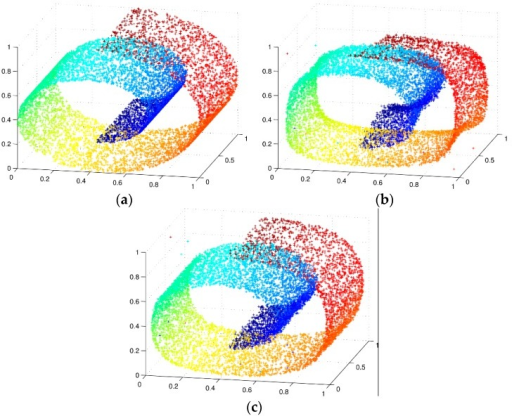
\includegraphics[scale=0.3]{swiss_roll.png}
    % swiss_roll.png: 512x416 px, 72dpi, 18.06x14.68 cm, bb=0 0 512 416
    \caption{An example of image inserted in report}
    \label{fig:swiss_roll}
\end{figure}
We have provided an image of the artificial data, \texttt{swiss roll} generated by our code in Figure~\ref{fig:swiss_roll}.

\begin{table}[h!t]
\caption{Table showing results}
{%
\newcommand{\mc}[3]{\multicolumn{#1}{#2}{#3}}
\begin{center}
\begin{tabular}{lccccc}
× & \mc{5}{c}{Methods}\\\cline{2-6}
\mc{1}{l}{Dataset} & \mc{1}{c}{None} & \mc{1}{c}{PCA} & \mc{1}{c}{KPCA} & \mc{1}{c}{Autoenc} & \mc{1}{c}{LLE}\\\hline
Swiss roll & 1 & 2 & 3 & 4 & 5\\
Broken Swiss & 6 & 7 & 8 & 9 & 10\\
Helix & 3 & 9 & 10 & 7 & 6\\
MNIST & 4 & 8 & 5 & 8 & 5\\
Olivetti face & 6 & 7 & 7 & 8 & 9
\end{tabular}
\end{center}
}%
\label{tab:results1}
\end{table} 
Table~\ref{tab:results1} summarises our results and will be discussed in Section~\ref{sec:discussion}


\section{Discussion}
\label{sec:discussion}
\lipsum[2]
\section{Conclusion}
\label{sec:conclusion}
\lipsum[9]
\bibliography{report_template}

\end{document}
